\section{Hardware design}

The central unit of the system is the BeagleBone Black single-board computer. This computer produced by Texas Instruments was chosen because it's high performance to cost ratio (important for Python) and it's extensive peripheral support.
The BeagleBone Black (BBB) is shipped with preinstalled Angström Linux, which is a lightweight Linux distribution developed for embedded devices. The advantages of using a linux distribution as an embedded operating system include the easy remote access to the system core via SSH, integrated package manager (opkg) with precompiled software distributions for the system (Python, bluez), and generally high community support.

The BBB doesn't contain any integrated sensors, but can be extended with Capes, specialized for different tasks. As the BMESHIP is in a prototype stage, only the most essential sensors will be installed, without the assistance of Capes.

The system contains only a small amount of electronics, assembled on a breadboard. The power to the BeagleBone is supplied from the 12V battery by a 5V voltage regulator IC through USB Cable.
Unfortunately the BeagleBone shuts down the USB devices if it’s powered through the regular 2.1 / 5.5 mm power cable, therefore we “trick” the device into thinking that it’s supplied from a regular usb device.

\begin{figure}[H]
	\centering
	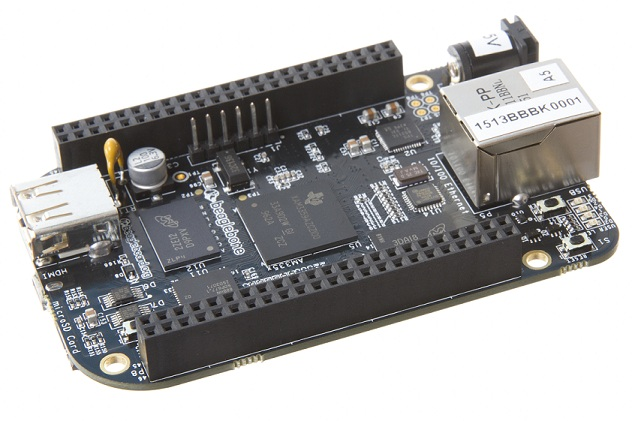
\includegraphics[width=1\textwidth]{img2/BeagleBone}
	\caption{The physical layout of the system}
	\label{fig:PhysicalLayout}
\end{figure}

Additional electronics include the motor controller board and the servo control, but unfortunately not all of the required parts are available yet.

\subsection{Remote control}

\subsection{Hardware}

\subsection{Assembly}